\documentclass[aspectratio=169,english]{beamer}

\usepackage[english]{babel}

\usepackage[T1]{fontenc}
\usepackage[utf8]{inputenc}
\usepackage{lmodern}
\usepackage{pgfplots}
\usepackage{xifthen}
\usepackage{newunicodechar}
\usepackage{textcomp}
\usepackage[absolute,overlay]{textpos}

\newunicodechar{°}{\textdegree}
\newunicodechar{µ}{\textmu}

\newcommand*{\ft}{\frametitle{\secname}}
\newcommand*{\ftsub}[1]{\frametitle{\secname\ - #1}}
\newcommand*{\itemp}{\item}
%\newcommand*{\itemp}{\pause\item}
\newcommand*{\+}{\texttt{+}}

\newcommand{\sectionframeimpl}[2]{
	\begin{frame}
	#1
	\begin{itemize}
	#2
	\end{itemize}
	\end{frame}
}
\newcommand{\sectionframe}[2]{
	\section{#1}
	\sectionframeimpl{\ft}{#2}
}
\newcommand{\subsectionframe}[2]{
%	\subsection{#1}
	\sectionframeimpl{\ftsub{#1}}{#2}
}
\newcommand{\subsubsectionframe}[2]{
%	\subsubsection{#1}
	\sectionframeimpl{\ftsub{#1}}{#2}
}

\beamertemplatenavigationsymbolsempty

\mode<presentation> {
%\usetheme{Berkeley}
%\usetheme{Goettingen}
%\usetheme{Hannover}
\usetheme{Madrid}

%\usetheme{default}
%\usetheme{AnnArbor}
%\usetheme{Antibes}
%\usetheme{Bergen}
%\usetheme{Berlin}
%\usetheme{Boadilla}
%\usetheme{boxes}
%\usetheme{CambridgeUS}
%\usetheme{Copenhagen}
%\usetheme{Darmstadt}
%\usetheme{Dresden}
%\usetheme{EastLansing}
%\usetheme{Frankfurt}
%\usetheme{Ilmenau}
%\usetheme{JuanLesPins}
%\usetheme{Luebeck}%\usetheme{Malmoe}
%\usetheme{Marburg}
%\usetheme{Montpellier}
%\usetheme{PaloAlto}
%\usetheme{Pittsburgh}
%\usetheme{Rochester}
%\usetheme{Singapore}
%\usetheme{Szeged}
%\usetheme{Warsaw}

%\usecolortheme{albatross}
%\usecolortheme{beaver}
%\usecolortheme{beetle}
%\usecolortheme{crane}
%\usecolortheme{default}
%\usecolortheme{dolphin}
%\usecolortheme{dove}
%\usecolortheme{fly}
%\usecolortheme{lily}
%\usecolortheme{monarca}
%\usecolortheme{orchid}
%\usecolortheme{rose}
%\usecolortheme{seagull}
%\usecolortheme{seahorse}
%\usecolortheme{sidebartab}
\usecolortheme{spruce}
%\usecolortheme{whale}
%\usecolortheme{wolverine}
}

\begin{document}

\title[Nouveau]{Project Overview \\ Nouveau \\ Open-source driver for Nvidia graphics card}
%\author{Karol Herbst}
\date{}

\begin{frame}
\titlepage
\end{frame}

\section*{Overview}

\begin{frame}
\ft
\tableofcontents
\end{frame}

\sectionframe{Motivation}{
	\itemp How does the hardware work
	\itemp Completely open alternative
	\itemp To have fun!
}

\sectionframe{General Facts}{
	\itemp MIT licensed
	\itemp Started in 2005
	\itemp Accepted in 2010 in Linux 2.6.33 as experimental
	\itemp Marked Stable in Linux 3.4
	\itemp NetBSD Port
	\itemp supports most Nvidia GPUs (Riva TNT up to Geforce 10 series and Tegra)
	\itemp Envytools for Reverse Engineering
}

\sectionframe{Features}{
	\itemp Kernel Modesetting (KMS)
	\itemp APIs
	\begin{itemize}
		\itemp OpenGL 4.3 (unofficial: 4.5)
		\itemp OpenGL ES 3.1
		\itemp D3D9
		\itemp XvMC
		\itemp VDPAU
	\end{itemize}
	\itemp Hwmon - Linux HW Monitoring
	\itemp Various Power Management features
	\itemp LED control!!!
	\itemp[!] not all features on all GPUs
}

\section{Reverse Engineering}
\subsectionframe{Hardware}{
	\itemp MMIO register
	\itemp Engines
	\begin{itemize}
		\itemp PDISP (Display Engine)
		\itemp PGRAPH (Rendering Engine)
		\itemp Video Engines
		\itemp PMU
		\itemp many more
	\end{itemize}
	\itemp ISAs
	\begin{itemize}
		\itemp shaders/CUDA cores
		\itemp fµc
	\end{itemize}
	\itemp GPIO / I²C devices
	\begin{itemize}
		\itemp Sensors
		\itemp Fans
		\itemp ...
	\end{itemize}
	\itemp Tool: mmiotrace and demmio
}

\subsectionframe{VBIOS}{
	\itemp Describes the GPU
	\itemp Meaning of Tables
	\itemp Changing values and monitoring for runtime changes
	\itemp Guessing
	\itemp Tool: nvbios
}

\subsectionframe{Software}{
	\itemp Nvidias
	\begin{itemize}
		\itemp OpenGL
		\itemp VDPAU (Linux API for video acceleration)
		\itemp OpenCL
	\end{itemize}
	\itemp[] Implementation
	\itemp various Command Line Tools
	\itemp Tool: valgrind-mmt
}

\section{Development}
\subsectionframe{Kernel driver}{
	\itemp Object-Oriented C Code
	\itemp Implements DRM APIs (Direct Rendering Manager)
	\begin{itemize}
		\itemp Display (via KMS - kernel modesetting)
		\itemp Access from Userspace
		\itemp Memory Management (TTM)
		\itemp Rendering
	\end{itemize}
	\itemp Hwmon
	\itemp Power Management
}

\subsectionframe{X11 Server Driver / 2D acceleration}{
	\itemp package: xf86-video-nouveau
	\itemp native 2D hardware acceleration
	\itemp OpenGL can be used instead as well (via xf86-video-modesetting)
}

\subsectionframe{Mesa / 3D acceleration}{
	\itemp OpenGL (ES)
	\begin{itemize}
		\itemp Implementation of Gallium API
		\itemp Implementation of new OpenGL(ES) Extensions
		\itemp codegen (Shader Compiler)
		\begin{itemize}
			\itemp SSA based backend compiler
			\itemp optimisation passes
			\itemp register allocation
		\end{itemize}
	\end{itemize}
	\itemp VDPAU
	\itemp OpenCL (WIP)
	\begin{itemize}
		\item SPIR-V -> nv50ir
	\end{itemize}
	\itemp Vulkan (TODO)
}

\subsectionframe{OpenGL}{
	\itemp Driver/Backend
	\itemp API
	\itemp Extensions
	\itemp Khronos CTS
}

\sectionframe{Working with Nvidia}{
	\itemp Announced to provide Documentation for basic features
	\begin{itemize}
		\itemp Some register documentation for Tegra K1
		\itemp basic VBIOS specs needed for Displays
		\itemp open-gpu-doc (partly helpful)
	\end{itemize}
	\itemp Open-Source Android Driver (will be replaced by Nouveau)
	\itemp Help paid Nouveau developer with hardware bugs
	\itemp Paid developers for Nvidia Tegra support
	\itemp Signed firmware for Maxwell2\+
}

\sectionframe{Biggest Challanges}{
	\itemp Pass Khronos CTS for exposing OpenGL 4.4\+
	\itemp Improving Performance
	\itemp Maxwell2\+
	\begin{itemize}
		\itemp Signed VBIOS
		\itemp Signed Firmware
		\itemp Required for accessing protected Registers
		\begin{itemize}
			\itemp Fan control
			\itemp Reclocking (since Pascal)
			\itemp Tons of stuff as well (since Pascal)
		\end{itemize}
		\itemp 128 bit AES key
		\itemp Harder REing of VBIOS and MMIO registers
		\pause\only<2>{
			\begin{textblock*}{5cm}(9cm,2.2cm)
				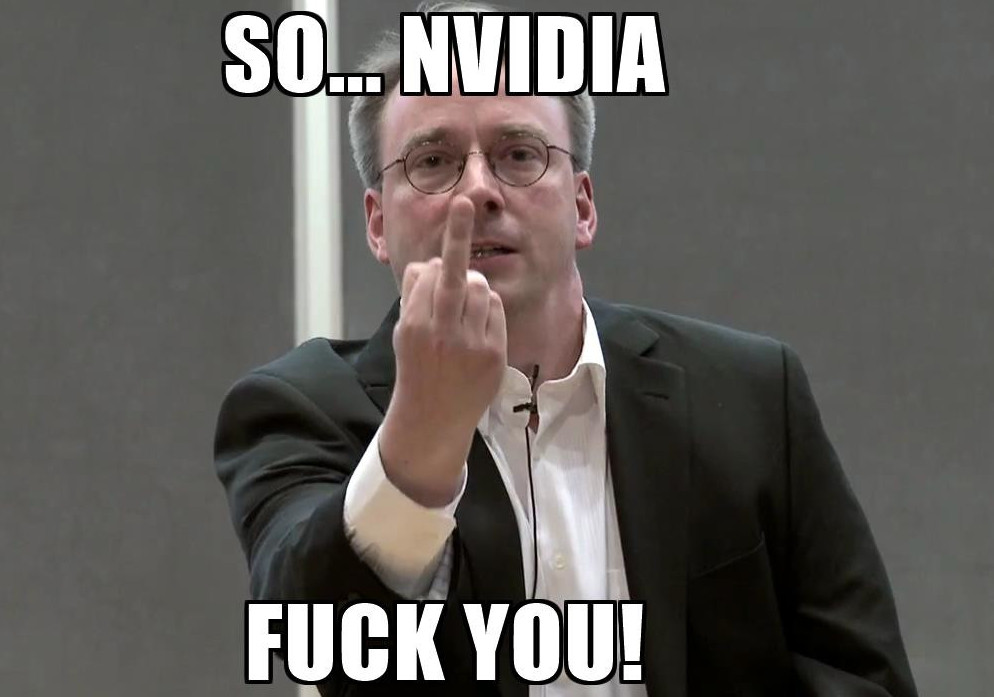
\includegraphics[scale=0.2]{linus}
			\end{textblock*}
		}
	\end{itemize}
}

\sectionframe{Links}{
	\item IRC Channel on freenode: \href{ircs://chat.freenode.net:6697/\#nouveau}{\#nouveau}
	\item Mailing list: \url{https://lists.freedesktop.org/mailman/listinfo/nouveau}
	\item Trello Board: \url{https://trello.com/b/ZudRDiTL/nouveau}
}

\end{document}